\section{Peer-to-Peer-Technologie}
\label{subsec:peer_to_peer_technologie}
% #TODO: Funktion des Kademlia Protokolls nennen und erklären (vielleicht in Grundlagen)
% Im Kademlia-Protokoll sind vier Funktionen definiert, die für die Suche nach
% Knoten und Werten verwendet werden. Diese Funktionen sind \texttt{FIND\_NODE},
% \texttt{FIND\_VALUE}, \texttt{PING} und \texttt{STORE}. Die Funktionen
% \texttt{FIND\_NODE} und \texttt{FIND\_VALUE} werden verwendet, um nach Knoten
% oder Werten zu suchen. Die Funktion \texttt{PING} wird verwendet, um die
% Erreichbarkeit eines Knotens zu überprüfen. Die Funktion \texttt{STORE} wird
% verwendet, um einen Wert in einem Knoten zu speichern.

% Was ist ein Peer-to-Peer-Netzwerk?
% Wie funktioniert es?
% Welche Typen gibt es?
% Welche Vorteile bietet es?
% Welche Nachteile gibt es?
% Welche Anwendungen gibt es?
% Welche Probleme gibt es bei Peer-to-Peer-Netzwerken?
% Welche Lösungen gibt es für diese Probleme?
% Welche Peer-to-Peer-Protokolle gibt es?
% Welche Peer-to-Peer-Protokolle werden in dieser Arbeit verwendet?

Peer-to-Peer bezeichnet ein Netzwerkmodell, bei dem Computer und andere Geräte direkt miteinander verbunden sind, um Ressourcen gemeinsam zu nutzen, ohne dass ein zentraler Server erforderlich ist. Bei diesem Netzwerkprotokoll sind alle Teilnehmer gleichberechtigt, es existiert kein zentraler Server, der die Kommunikation steuert. Die Kommunikation erfolgt direkt zwischen den Teilnehmern, die in einem Netzwerk aus verschiedenen Knoten organisiert sind. Jeder Knoten repräsentiert dabei einen Teilnehmer des Netzwerks und ermöglicht den direkten Austausch von Textnachrichten und Dateien zwischen den verbundenen Knoten \parencite[S. 6-8]{Mahlmann_P2PNetzwerke}.

Viele werden Peer-to-Peer schnell mit Filesharing in Verbindung bringen, da diese Technologie in der Vergangenheit vor allem dafür genutzt wurde. Das bekannteste Beispiel ist das Filesharing-Netzwerk Napster, das 1999 von Shawn \enquote{Napster} Fanning entwickelt wurde. Napster war das erste weit verbreitete Filesharing-Netzwerk, das auf Peer-to-Peer-Technologie basierte. Es ermöglichte den Austausch von Musikdateien zwischen den Teilnehmern. Die Musikdateien wurden dabei auf den Computern der Teilnehmer gespeichert und konnten von anderen Teilnehmern heruntergeladen werden. Da diese Art des Datenaustauschs oftmals illegal war, wurde Napster 2001 aufgrund von Urheberrechtsverletzungen abgeschaltet \parencite[S. 4-6]{Mahlmann_P2PNetzwerke}.


Im Bereich des Instant-Messaging ist Peer-to-Peer ein dezentrales Kommunikationsmodell, bei dem alle Teilnehmer gleichberechtigt sind und sowohl als Client als auch als Server fungieren können. Im Gegensatz zu einem Client-Server-Modell, bei dem ein zentraler Server die Kommunikation zwischen den Teilnehmern verwaltet, kommunizieren die Teilnehmer in einem Peer-to-Peer-Netzwerk direkt miteinander. Dieses Modell bietet eine Reihe von Vorteilen, wie z.B. eine höhere Skalierbarkeit, da die Last auf mehrere Teilnehmer verteilt wird, und eine höhere Ausfallsicherheit, da das Netzwerk nicht von einem zentralen Server abhängig ist. Server können in Problemfällen zu einem Single Point of Failure werden, der das gesamte Netzwerk beeinträchtigen kann, wenn er ausfällt. Ein weiterer Vorteil ist die höhere Privatsphäre, da die Kommunikation direkt zwischen den Teilnehmern erfolgt und nicht über einen zentralen Server, der die Kommunikation überwachen könnte. Allerdings ist die Kommunikation in einem Peer-to-Peer-Netzwerk schwieriger zu verwalten, da es keine zentrale Instanz gibt, die die Kommunikation überwacht und verwaltet. Außerdem ist die Identifizierung der Teilnehmer schwieriger, da es keine zentrale Instanz gibt, die die Teilnehmer verwaltet. Dieses Problem kann durch die Verwendung eines strukturierten Peer-to-Peer-Netzwerks gelöst werden, das eine explizite Organisationsstruktur für die Teilnehmer bietet, um die Suche und Verwaltung zu erleichtern \parencite[S. 6-8]{Mahlmann_P2PNetzwerke}.

Die Nutzung einer zentralen Instanz birgt das Risiko eines Single Points of Failure, welcher das gesamte Netzwerk beeinträchtigen kann, falls er ausfällt. Trotzdem bietet ein zentrales System Vorteile, da die Identifizierung der Teilnehmer einfacher ist, da eine zentrale Instanz für das Management verantwortlich ist. Im Gegensatz dazu sind Peer-to-Peer-Netzwerke schwerer zu zensieren, da keine zentrale Instanz existiert, die zensiert werden könnte. Allerdings gestaltet sich die Suche und Verwaltung der Teilnehmer im Peer-to-Peer-Modell schwieriger ohne das Vorhandensein eines Servers. Dieses Problem kann durch die Verwendung eines strukturierten Peer-to-Peer-Netzwerks gelöst werden, das eine explizite Organisationsstruktur für die Teilnehmer bietet, um die Suche und Verwaltung zu erleichtern \parencite{Luntovskyy_ModRechnernetze}.

\begin{center}
    \captionsetup{type=figure}
    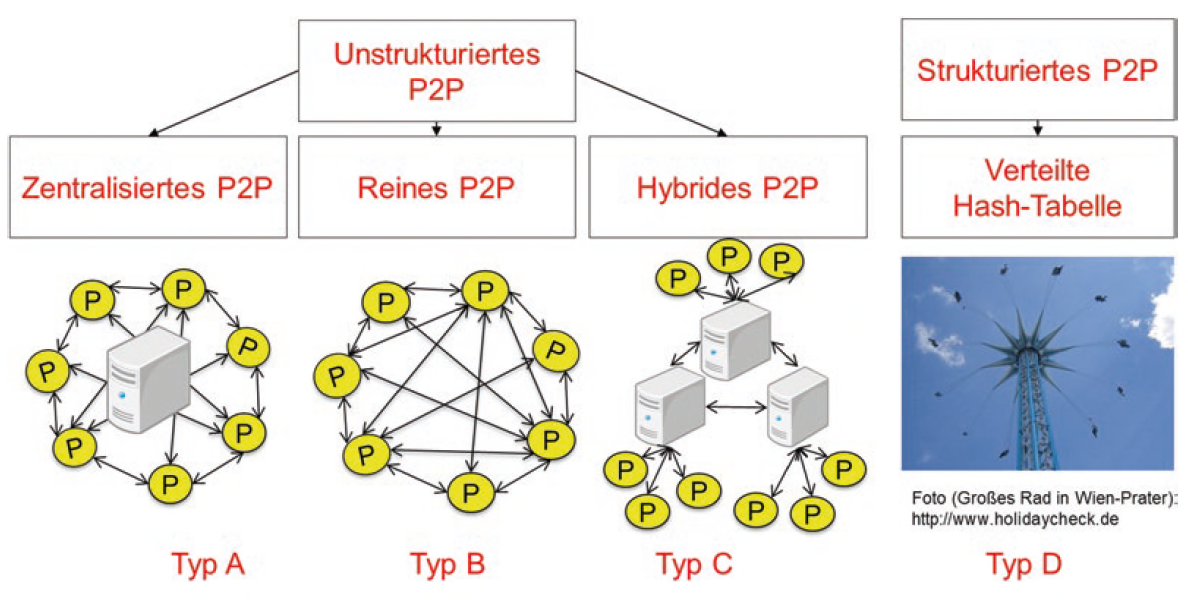
\includegraphics[width=1\linewidth]{images/peer_to_peer_typen.png}
    \captionof{figure}{Typen von Peer-to-Peer-Netzwerken \parencite{Luntovskyy_ModRechnernetze}}
    \label{p2p_typen}
\end{center}

\noindent Unstrukturierte, strukturierte und hybride Peer-to-Peer-Netzwerke sind unterschiedliche Ansätze zur Organisation von Knoten und Ressourcen in dezentralen Netzwerken. Unstrukturierte Netzwerke sind charakterisiert durch ihre fehlende explizite Organisationsstruktur, was eine einfache Konnektivität ermöglicht. Diese Netzwerke sind dynamisch und erlauben es Knoten frei beizutreten oder das Netzwerk zu verlassen, ohne die Gesamtstruktur signifikant zu beeinflussen. Die Suche nach Ressourcen oder Informationen erfolgt oft durch Broadcasts oder zufällige Weiterleitungen, was jedoch zu ineffizienten Suchprozessen führen kann, da keine klare Routing-Struktur vorhanden ist. Ein klassisches Beispiel für ein unstrukturiertes Netzwerk ist das Gnutella-Netzwerk, das sich durch seine dezentrale Natur auszeichnet, jedoch bei der effizienten Ressourcenlokalisierung Schwierigkeiten aufgrund des fehlenden organisierten Routings hat \textcolor{red}{[QUELLE]}.

Strukturierte Peer-to-Peer-Netzwerke hingegen weisen klare Regeln und Algorithmen zur Organisation der Knoten auf. Diese Netzwerke verfügen über eine explizite Organisationsstruktur, sei es eine Ringstruktur, k-bucket basierte Systeme oder andere, die es ermöglichen, effizientes Routing und eine optimierte Ressourcenverwaltung zu erreichen. Durch diese klar definierte Struktur sind strukturierte Netzwerke oft stabiler und bieten eine effizientere Ressourcenlokalisierung im Vergleich zu ihren unstrukturierten Gegenstücken. Allerdings kann diese Stabilität auf Kosten von Flexibilität und Anpassungsfähigkeit gehen, da Änderungen in der Netzwerktopologie oder hohe Dynamik der Knoten schwerer zu handhaben sind \textcolor{red}{[QUELLE]}.

Hybride Peer-to-Peer-Netzwerke versuchen, das Beste aus beiden Welten zu vereinen, indem sie Elemente aus strukturierten und unstrukturierten Ansätzen kombinieren. Diese Netzwerke integrieren Aspekte einer festen Organisationsstruktur für bestimmte Netzwerkbereiche, während andere Bereiche eher unstrukturiert sind. Als Beispiel hierfür kann Napster genannt werden, das eine oder mehrere Nodes dazu verwendet, um die Inhalte innerhalb des Netzwerks zu indizieren und zu verwalten, während der tatsächliche Download des Inhalts über eine direkte Verbindung zwischen den Teilnehmern erfolgt \parencite{Yang_ComparingHybridP2PSystems}.
Ziel ist es, Flexibilität und Effizienz zu optimieren und gleichzeitig eine gewisse Stabilität zu gewährleisten. Diese hybriden Ansätze streben danach, eine ausgewogene Lösung zu bieten, die sowohl die Anforderungen an eine stabile Struktur als auch an eine dynamische und flexible Umgebung erfüllt, je nach den spezifischen Bedürfnissen und Anwendungsfällen \textcolor{red}{[QUELLE]}.





\begin{itemize}
    \item NAT-Problem erklären (siehe RFC 5128)
    \item Mögliche Lösungen des NAT-Problems (siehe RFC 5128)
    \item Kademlia-Protokoll und DHTs erklären
    \item STUN, TURN und ICE erklären (je nach dem, was ich davon verwende)
\end{itemize}